\documentclass[11pt]{thyv}

\usepackage[utf8]{inputenc}
\RequirePackage[T1]{fontenc}
\usepackage{xcolor}
\usepackage{tikz}
\usepackage{graphicx}
\usepackage{amsmath}
\usepackage{marvosym}
\usepackage{relsize}
\usepackage{doi}
\usepackage{url}
\usepackage{hyperref}

\begin{document}

	\begin{tikzpicture}[remember picture,overlay]
   		\node [rectangle, anchor=north, minimum width=6cm, minimum height=\paperheight+1cm] (box) at (-5cm,1.5cm){};
	\end{tikzpicture}

	%------------------------------------------------

	\begin{textblock}{5}(0.5, 0)

		%------------------------------------------------

		
			\begin{center}
				\begin{tikzpicture}[x=\imagescale,y=-\imagescale]
					\clip (300, 300) circle (300);
					\draw[line width=2pt] (300, 300) circle (300);
					\node[anchor=north west, inner sep=0pt, outer sep=0pt] at (0,0) {
						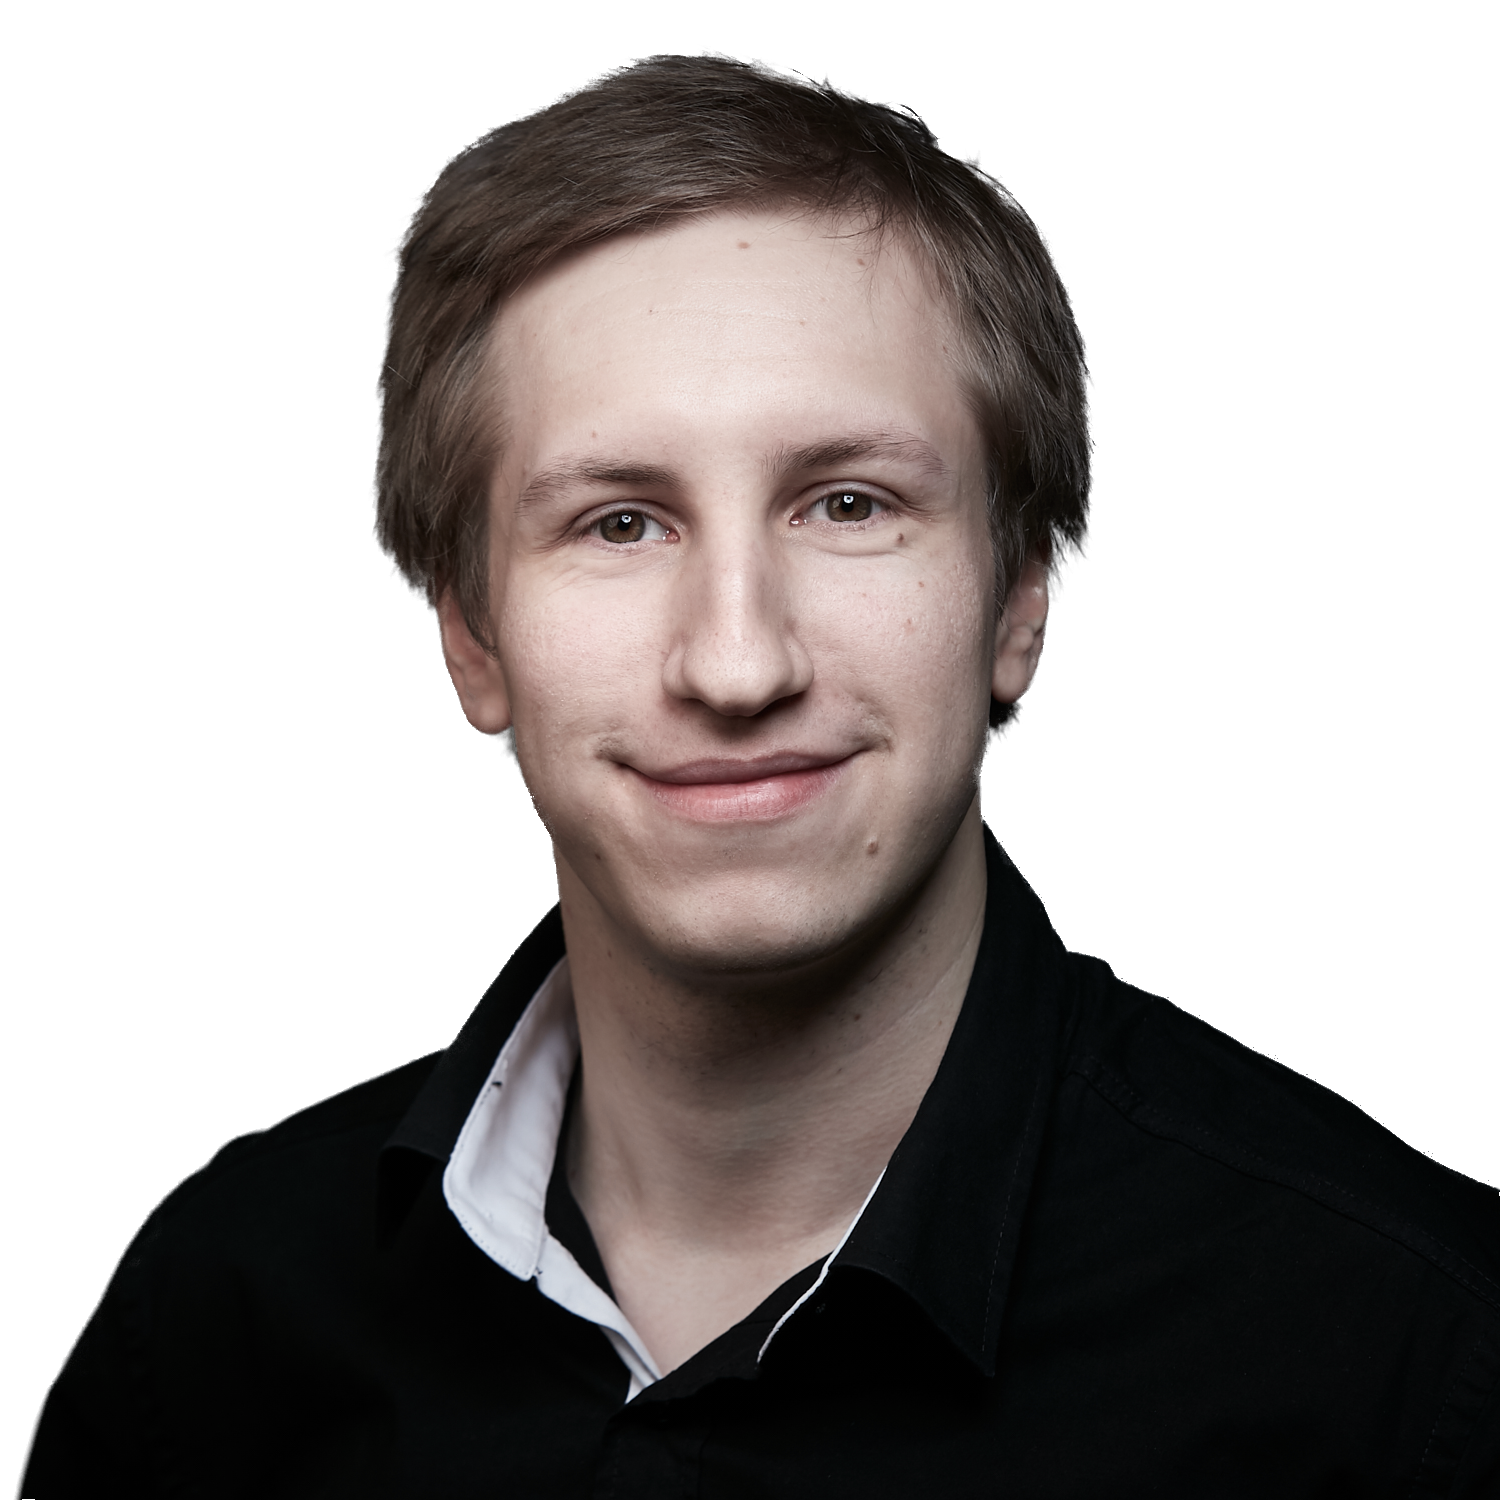
\includegraphics[width=\imagewidth]{max0.6.png}
					};
				\end{tikzpicture}
			\end{center}
		

		%------------------------------------------------


		{\Large Max-Jonathan Luckow}

		%------------------------------------------------

		{Computer Science Student}

		\strut

	\begin{thyV}{2010}{2024}{21}{0.6\linewidth}
		\thyVent{high-school\\ diploma} 				{6/2010}
		\thyVent{Publication} 							{1/2020}
		\thyVent{B.Sc.\\Thesis} 						{3/2017}
		\thyVent{\\ M.Sc.Thesis} 						{3/2023}
		
		\thyVentEdu{Energy and\\Process Engineering} 	{4/2011}{9/2013} 	{}
		\thyVentEdu{Bachelor of Science \\Computer Science} 			{10/2013}{3/2017} 	{16.625/2014} 
		\thyVentEdu{Master of Science \\ Computer Science} 			{4/2017}{3/2023} 	{7.25/2020}

		\thyVentWork{Technical\\Accountant} 			{9/2020}{4/2022} 	{}
		\thyVentWork{Web Developer} 					{3/2018}{4/2018} 	{}
		\thyVentWork{Technical Specialist} 				{6/2017}{11/2017} 	{9.25/2017}
		\thyVentWork{Self-employed} 					{1/2014}{5/2017} 	{22.875/2014}

		\thyVentWork{Assistant in \\ surgical ward} 	{8/2010}{1/2011} 	{12.25/2010}
	\end{thyV}

		\thyLegend{Experience}{1.8cm}{thySecond} \thyLegend{Education}{1.8cm}{thyFirst} \thyLegend{Events}{1.1cm}{thyThird}
		%\parbox{2cm}{{\rule{1.5cm}{3pt}}\\Education}
		%\parbox{2cm}{{\rule{1.5cm}{3pt}}\\Experience}
		%\parbox{2cm}{{\rule{1.5cm}{3pt}}\\Experience}
		
		\begin{tabular}{lll}
		{\rule{1.5cm}{3pt}} & {\rule{1.5cm}{3pt}} & {\rule{1.5cm}{3pt}} \\
		Education & Experience & Events
		\end{tabular}

	\end{textblock}

	\begin{mdframed}

		\begin{minipage}[t]{0.50\textwidth} % 27.5% of the page width for the first row of icons
			\vspace{-\baselineskip} % Required for vertically aligning minipages

			\icon{Cross}{12}{30. November 1990}\\
			\icon{Phone}{12}{+49 163 222 99 64}\\
				
		\end{minipage}
		\begin{minipage}[t]{0.50\textwidth} 
			\vspace{-\baselineskip} % Required for vertically aligning minipages
			
			\icon{At}{12}{\href{mailto:max@luckow.ch}{max@luckow.ch}}\\
			\icon{Github}{12}{\href{https://github.com/Carlisle96}{github.com/Carlisle96}}\\
		\end{minipage}


		\section{Publication}
			M. J. Luckow and T. Fluschnik. \textbf{``\href{https://doi.org/10.1016/j.ipl.2019.105913}{On the Computational Complexity of Length- and Neighborhood-Constrained Path Problems}''}. In: \textit{Information Processing Letters.} Vol. 156 (2020). %\texttt{\doi{10.1016/j.ipl.2019.105913}}

		\section{Work Experience}

			\textbf{Technical Acountant} at \textbf{Agilo-Services GmbH}				\hfill \textbf{09/2020 - Present}
				\begin{loneinnerlist}
					\item Analysis, optimization, automation and supervision of the accounting system
				\end{loneinnerlist}

			\bigskip
			\textbf{Web Developer} at \textbf{Trado GmbH}								\hfill \textbf{03/2018 - 04/2018}
				\begin{loneinnerlist}
					\item Programming and maintenance of the internal administrative software
				\end{loneinnerlist}

			\bigskip
			\textbf{Technical Specialist} at \textbf{Envion AG} 						\hfill \textbf{06/2017 - 11/2017}
			    \begin{loneinnerlist}
			    	\item Analysis of Cryptocurrency market
			    	\item Devolopment of the first mining operations prototype
			    	\item Supervision of the production of the first large scale mining operation
			    \end{loneinnerlist}

			\bigskip
			\textbf{Self-employed} 														\hfill \textbf{01/2014 - 05/2017}
			    \begin{loneinnerlist}
			    	\item IT administration, development and project support
			    \end{loneinnerlist}

		\section{Education}

			\textbf{Technical University of Berlin}

			\begin{outerlist}
				\item[] Master of Science. \textit{Computer Science} 					\hfill \textbf{04/2017 - \textit{03/2023}}
				        \begin{innerlist}
				        	\item Specialisation in: Cognitive Systems
				        \end{innerlist}

				\item[] Bachelor of Science. \textit{Computer Science} 					\hfill \textbf{10/2013 - 03/2017}
				        \begin{innerlist}
				        \item Thesis: Algorithms and Complexity 						\hfill ( Grade 2.0 ) \\
				        Advisor: Prof. Dr. Rolf Niedermeier
				        \item Degree: Bachelor of Science 								\hfill ( Grade 2.8 ) \\
				        Area of Study: Foundations of Computing
				        \end{innerlist}

				\item[] Bachelor of Science. \textit{Energy and Process Engineering} 	\hfill \textbf{04/2011 - 09/2013}
			\end{outerlist}

			\bigskip
			\textbf{Arndt Gynasium Dahlem} 												\hfill \textbf{08/2003 - 06/2010}
			    \begin{outerlist}
			    	\item[] Degree: high-school diploma 								\hfill ( Grade 2.1 )
			    \end{outerlist}

		\section{Social Experience}

			\textbf{Hospital Waldfriede Berlin} 										\hfill \textbf{08/2010 - 01/2011}
			    \begin{outerlist}
			    	\item[] Community service in the surgial ward
			    \end{outerlist}

		\section{Technical Expertise}

			%\begin{multicols}{2}
			C/\Cplusplus, Java, Python \hfill \ThreeOfFour \\
			Latex \hfill \ThreeOfFour \\
			Haskell \hfill \OneOfFour \\
			Linux \hfill \TwoOfFour \\
			Solidity \hfill \TwoOfFour \\
			Javascript, Vue.js, Node.js, SQL \hfill \TwoOfFour \\
			%\vfill\null
			%\columnbreak
			Datev Uno \hfill \FourOfFour


			%\end{multicols}

		\section{Language Expertise}
			German \hfill Native speaker \\
			English \hfill Advanced \\
			Latin \hfill Latinum


		\hfill
\includegraphics[width=100pt]{signature2.png}
	\end{mdframed}




\end{document}